\chapter{Organisatorische Projektführung}

Die organisatorische Projektführung besteht aus folgenden Elementen:
\begin{description}
	\item[Projektorganisation:] Festlegen der Organisation und Gremien in einem Projekt.
	\item[Rollen und Kompetenzen:] Festlegen der Rollen und deren Kompetenzen in einem Projekt z.B. IT- und Business Projektleiter.
	\item[Projektstruktur(plan):] Aufteilung eines Projektes in Teilprojekte oder Streams.
\end{description}

\section{Projektorganisation}
In der Abbildung \ref{fig:projekt-organisation} ist eine typische Projekt-Organisation abgebildet.

\begin{figure}[h!]
\centering
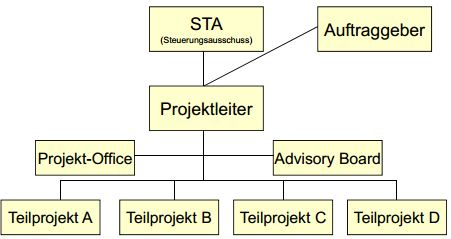
\includegraphics[width=0.7\linewidth]{fig/projekt-organisation}
\caption{Projekt-Organisation}
\label{fig:projekt-organisation}
\end{figure}

\section{Rollen}
Eine solche Organisation umfasst verschiedene Rollen:
\begin{description}
	\item[Projektleiter PL:] Führt und ''managed'' das Projekt. Jedes Projekt hat einen gesamtverantwortlichen Projektleiter. Verantwortlich für Resultate und erfolgreiche Durchführung.
	\item[Auftraggeber:] Der Sponsor überwacht das Projekt und trägt die volle Projektverantwortung, auch wenn er seine Aufgaben oder Kompetenzen teilweise delegiert (an PL oder STA).
	\item[Steuerungsausschuss (STA):] Kontrolliert und ''steuert'' das Projekt. Er gibt Budgets frei, nimmt Meilensteine ab oder entscheidet über die Weiterführung oder Abbruch. Unterstützt den Auftraggeber und tagt periodisch.
	\item[Teilprojektleiter:] Verantwortlich für ein klar abgegrenzter Teilbereich (Teilprojekt). Dieser hat für das Teilprojekt in etwa die gleichen Aufgaben und Kompetenzen wie ein Projektleiter.
	\item[Projekt-Office:] In jedem Projekt braucht es Sekretärinnen, welche administrative Aufgaben übernehmen. Es zählen folgende dazu: Meetings organisieren, Termine überwachen, Issuelisten führen, Kontrolle des Projektfortschritts.
	\item[Advisory Board:] Das Board besteht aus Experten, Schlüsselpersonen und Kunden des Projekts. Es ''berät'' das Projekt, gibt Feedbacks zu Lösungen und ist ein wichtiges Bindeglied zu den Benutzern. Es hat jedoch keine Entscheidungskompetenzen.
\end{description}

\section{Projektstrukturierung}
\label{sec:projektstrukturierung}
Eine Projektstrukturierung legt fest nach welchen Kriterien ein Projekt in Teilprojekte oder Streams unterteilt wird. Diese Struktur wird meist in einem Projektstrukturplan festgehalten. Folgendes sind Kriterien für eine Projektstrukturierung:
\begin{itemize}
	\item Grösse und Komplexität des Projektes
	\item Ausrichtung nach Resultaten oder Phasen
	\item Entkopplungsgrad der Teilprojekte und Parallelisierbarkeit der Arbeiten
	\item Zentralisierung oder Dezentralisierung von Verantwortung und Kompetenzen (Teilprojekte vs Streams)
	\item Geeignetes Personal: Verfügbarkeit von geeigneten TP-Leiter.
\end{itemize}

\subsection{Phasen- vs. ergebnisorientiert}
Wie in SoDa (Phasen \& Komponenten). Entweder strukturiert man das Projekt nach Phasen (Führung, Initialisierung, Konzeption, Realisierung, Einführung) oder nach Ergebnissen (Bsp: Weltreise - Transport, Übernachtung, Sehenswürdigkeiten, Verpflegung).

\subsection{Teilprojekte vs. Streams}
\begin{description}
	\item[Teilprojekt] Umfasst alle Elemente eines normalen Projekts. Ein TP-Leiter hat die volle Resultatverantwortung mit allen notwendigen Kompetenzen und Aufgaben wie Projektplanung, Budget, Controlling und Reporting.
	\item[Stream] Ein Stream ist ein Teilprojekt OHNE Resultatverantwortung und OHNE die klassischen Projektführungsaufgaben. Beides ist Aufgabe des PL!
\end{description}

\section{Lernziele}
\subsection{Sie kennen die Kriterien für die Definition einer Projektstruktur}
Siehe Abschnitt \ref{sec:projektstrukturierung}

\subsection{Sie können eine Projektstruktur definieren und begründen}
Siehe Abschnitt \ref{sec:projektstrukturierung}